\documentclass{beamer}
\usepackage{forest}
\usepackage{proof}
\usepackage{minted}
\usepackage{makecell}
\usepackage{changepage}
\newcommand{\NL}[0]{ \hfill\\\noindent }
\newcommand{\coloneqtwo}{\mathbin{:\hspace{-0.5ex}\textsf{-}}}

\newcommand{\strconst}[1]{ \colorbox{green!10}{#1} }
\newcommand{\predconst}[1]{ \colorbox{blue!10}{#1} }
\newcommand{\intconst}[1]{ \colorbox{cyan!10}{#1} }
\newcommand{\listconst}[1]{ \colorbox{orange!10}{#1} }
\newcommand{\typeconst}[1]{ \colorbox{red!10}{#1} }
\begin{document}	
\begin{frame}
% \frametitle{Datalog - Recursive Query Processing}

\begin{center}
	\Huge Datalog \\
	\huge Recursive Query Processing
\end{center}
%Content goes here
\end{frame}


\begin{frame}
\frametitle{Basic Idea}
\begin{itemize}
\item<1->  Datalog uses first-order logic to express relations \textit{(Relation = Table = Predicate)}
\item<2->  Start with some facts (also called EDBs for extensional database): 
\end{itemize}
\uncover<2->{
\begin{align*}
&Parent(\strconst{"Eddard"}, \strconst{"Arya"}).\\
&Parent(\strconst{"Lyarra"}, \strconst{"Eddard"}).\\
\end{align*}
}
\vspace*{-1.2cm}
\begin{itemize}
\item<3->  State some rules and derive new facts: 
\end{itemize}
\uncover<3->{
\begin{align*}
&Ancestor(p, c) \coloneqtwo Parent(p, c).\\
&Ancestor(a, c) \coloneqtwo Parent(p, c), Ancestor(a, p).\\
\end{align*}
}
\vspace*{-1.2cm}
\begin{itemize}
\item<4->  Semantics: Right-hand side implies left-hand side
\end{itemize}
\end{frame}
%\begin{frame}
%\frametitle{The core Datalog language}
%\framesubtitle{A bit more information about this}
%A Datalog program is a set of rules.\NL

%\begin{itemize}
%\item<1-> \fbox{$Ancestor(a, c) \coloneqtwo Parent(p, c), Ancestor(a, p).$} \hfill Rule
%\item<2-> $\fbox{Ancestor(a, c)} \coloneqtwo \fbox{Parent(p, c), Ancestor(a, p)}.$ \hfill Head, Body
%\item<3-> \fbox{$Ancestor(a, c)$} \hfill Atom
%\item<4-> \fbox{$Ancestor$}(\fbox{$a, c$}) \hfill Predicate, List of Terms
%\item<5-> A term is a variable or a constant.
%\item<6->Semantics (implication from body to head): \\
%	$\forall Constants\;(\strconst{p},\strconst{c},\strconst{a}).$\\ 
%	\hspace*{15 pt} 
%	$Parent(\strconst{p}, \strconst{c}) \land Ancestor(\strconst{a}, \strconst{p}) \implies Ancestor(\strconst{a},\strconst{c})$
%\end{itemize}
%More content goes here
%\end{frame}

%\begin{frame}
%\frametitle{EDBs and IDBs}
%\begin{itemize}
%\item<2-> \textbf{EDB: } Extensional database, explicitly defines predicates through facts.
%\item<4-> \textbf{IDB: } Intensional database, implicitly defines predicates through rules (Horn Clauses) showing intent.
%\end{itemize}
%\NL
%\uncover<3,6>{$Parent(\strconst{"Eddard"}, \strconst{"Arya"}).$}\NL
%\uncover<3,6>{$Parent(\strconst{"Lyarra"}, \strconst{"Eddard"}).$}\NL
%\NL
%\uncover<5-6>{$Ancestor(p, c) \coloneqtwo Parent(p, c).$}\NL
%\uncover<5-6>{$Ancestor(a, c) \coloneqtwo Parent(p, c), Ancestor(a, p).$}
%\end{frame}

\begin{frame}
\frametitle{Fix-point Iteration}
\framesubtitle{How to derive facts?}
\begin{itemize}
\item<1-> Begin with the EDB facts: $I^0$.
\end{itemize}
\vspace*{-0.5cm}
\uncover<2->{
	\hspace*{-5cm}
\begin{align*}
&Parent(\strconst{"Eddard"}, \strconst{"Arya"}).\\
&Parent(\strconst{"Lyarra"}, \strconst{"Eddard"}).\\
\end{align*}
}
\vspace*{-1.2cm}
\begin{itemize}
\item<3-> Iterate rules until no new tuples can be derived, $I^0, I^1, \ldots, I^n = I^{n + 1}$
\end{itemize}
\vspace*{-0.2cm}
\uncover<3->{
	\centering
\begin{align*}
&Ancestor(p, c) \impliedby Parent(p, c).\\
&Ancestor(a, c) \impliedby Parent(p, c) \land Ancestor(a, p).\\
\end{align*}
}
\vspace*{-1.0cm}
\begin{itemize}
\item<4-> Guaranteed termination with finite EDBs (and without object creation)!
\end{itemize}
%	\item<7->  \textbf{Naive evaluation}: use $I^{i + 1}$ as input to each iteration.
%\item<7->  \textbf{Semi-Naive evaluation}: use $\Delta_i$ as input to each iteration.
%Naive evaluation is less efficient than semi-naive evaluation

\end{frame}
\iffalse
\begin{frame}
\frametitle{Fix-point Iteration}
\framesubtitle{Example continued}
\uncover<2->{EDBs:}\NL
\uncover<1-2>{$Parent(\strconst{"Eddard"}, \strconst{"Arya"}).$}\NL
\uncover<1-2>{$Parent(\strconst{"Lyarra"}, \strconst{"Eddard"}).$}\NL
\NL
\uncover<1-1>{$Ancestor(p, c) \coloneqtwo Parent(p, c).$}\NL
\uncover<1-1>{$Ancestor(a, c) \coloneqtwo Parent(p, c), Ancestor(a, p).$}

\uncover<2->{
Database $I^0$:\NL\NL
\begin{tabular}{ | c | c | }
	\hline
	\multicolumn{2}{|c|}{\textbf{Parent}}\\
	\hline
	\textbf{p}  & \textbf{ c }\\
	\hline
	\strconst{"Eddard"}  & \strconst{"Arya"}\\
	\hline
	\strconst{"Lyarra"}  & \strconst{"Eddard"}\\
	\hline
\end{tabular}
\begin{tabular}{ | c | c | }
	\hline
	\multicolumn{2}{|c|}{\textbf{Ancestor}}\\
	\hline
	\textbf{a}  & \textbf{ c }\\
	\hline
\end{tabular}
}

\end{frame}

\begin{frame}
\frametitle{Fix-point Iteration}
\framesubtitle{Example continued}
\uncover<1->{
	Database $I^0$:\NL\NL
	\begin{tabular}{ | c | c | }
		\hline
		\multicolumn{2}{|c|}{\textbf{Parent}}\\
		\hline
		\textbf{p}  & \textbf{ c }\\
		\hline
		\strconst{"Eddard"}  & \strconst{"Arya"}\\
		\hline
		\strconst{"Lyarra"}  & \strconst{"Eddard"}\\
		\hline
	\end{tabular}
	\begin{tabular}{ | c | c | }
		\hline
		\multicolumn{2}{|c|}{\textbf{Ancestor}}\\
		\hline
		\textbf{a}  & \textbf{ c }\\
		\hline
	\end{tabular}
}
\NL\NL
\uncover<2->{Apply: $Ancestor(p, c) \coloneqtwo Parent(p, c).$}\NL

\uncover<3->{
	Database $I^1$:\NL\NL
	\begin{tabular}{ | c | c | }
		\hline
		\multicolumn{2}{|c|}{\textbf{Parent}}\\
		\hline
		\textbf{p}  & \textbf{ c }\\
		\hline
		\strconst{"Eddard"}  & \strconst{"Arya"}\\
		\hline
		\strconst{"Lyarra"}  & \strconst{"Eddard"}\\
		\hline
	\end{tabular}
	\begin{tabular}{ | c | c | }
		\hline
		\multicolumn{2}{|c|}{\textbf{Ancestor}}\\
		\hline
        \textbf{a}  & \textbf{ c }\\
		\hline
		\strconst{"Eddard"}  & \strconst{"Arya"}\\
		\hline
		\strconst{"Lyarra"}  & \strconst{"Eddard"}\\
		\hline
	\end{tabular}
}

\end{frame}
\begin{frame}
\frametitle{Fix-point Iteration}
\framesubtitle{Example continued}
\uncover<1->{
	Database $I^1$:\NL\NL
\begin{tabular}{ | c | c | }
	\hline
	\multicolumn{2}{|c|}{\textbf{Parent}}\\
	\hline
	\textbf{p}  & \textbf{ c }\\
	\hline
	\strconst{"Eddard"}  & \strconst{"Arya"}\\
	\hline
	\strconst{"Lyarra"}  & \strconst{"Eddard"}\\
	\hline
\end{tabular}
\begin{tabular}{ | c | c | }
	\hline
	\multicolumn{2}{|c|}{\textbf{Ancestor}}\\
	\hline
	\textbf{a}  & \textbf{ c }\\
	\hline
	\strconst{"Eddard"}  & \strconst{"Arya"}\\
	\hline
	\strconst{"Lyarra"}  & \strconst{"Eddard"}\\
	\hline
\end{tabular}
}
\NL\NL
\uncover<2->{Apply: $Ancestor(a, c) \coloneqtwo Parent(p, c), Ancestor(a, p).$}\NL

\uncover<3->{
	Database $I^2$:\NL\NL
	\begin{tabular}{ | c | c | }
		\hline
		\multicolumn{2}{|c|}{\textbf{Parent}}\\
		\hline
		\textbf{p}  & \textbf{ c }\\
		\hline
		\strconst{"Eddard"}  & \strconst{"Arya"}\\
		\hline
		\strconst{"Lyarra"}  & \strconst{"Eddard"}\\
		\hline
	\end{tabular}
	\begin{tabular}{ | c | c | }
		\hline
		\multicolumn{2}{|c|}{\textbf{Ancestor}}\\
		\hline
		\textbf{a}  & \textbf{ c }\\
		\hline
		\strconst{"Eddard"}  & \strconst{"Arya"}\\
		\hline
		\strconst{"Lyarra"}  & \strconst{"Eddard"}\\
		\hline
		\strconst{"Lyarra"}  & \strconst{"Arya"}\\
		\hline
	\end{tabular}
}

\end{frame}
\begin{frame}
\frametitle{Fix-point Iteration}
\framesubtitle{Example continued}
\uncover<1->{
	Database $I^2 = I^3$:\NL\NL
\begin{tabular}{ | c | c | }
	\hline
	\multicolumn{2}{|c|}{\textbf{Parent}}\\
	\hline
	\textbf{p}  & \textbf{ c }\\
	\hline
	\strconst{"Eddard"}  & \strconst{"Arya"}\\
	\hline
	\strconst{"Lyarra"}  & \strconst{"Eddard"}\\
	\hline
\end{tabular}
\begin{tabular}{ | c | c | }
	\hline
	\multicolumn{2}{|c|}{\textbf{Ancestor}}\\
	\hline
	\textbf{a}  & \textbf{ c }\\
	\hline
	\strconst{"Eddard"}  & \strconst{"Arya"}\\
	\hline
	\strconst{"Lyarra"}  & \strconst{"Eddard"}\\
	\hline
	\strconst{"Lyarra"}  & \strconst{"Arya"}\\
	\hline
\end{tabular}
}
\NL\NL
\uncover<2->{Iterating rules again gives no new tuples. \\A fix-point has been reached.}
\end{frame}
\fi

\begin{frame}
\frametitle{Language Extensions}
Extend the expressive power of core Datalog.
\begin{itemize}
\item<2-> Negation: \\
$LivingPerson(p) \coloneqtwo Person(p), NOT(Dead(p)).$

\item<3-> Object Generation with BIND:\\
$Nat(0).$\\
$Nat(y) \coloneqtwo Nat(x), BIND(y, x + \intconst{1}).$

\item<4-> Filtering: \\
$Nat(y) \coloneqtwo Nat(x), BIND(y, x + \intconst{1}), y \leq \intconst{1000}$
\item<5-> Predicate References: \\
$OUTPUT(\predconst{'Parent}).$
\item<6-> Types (and Lists): \\
TYPEOF(\predconst{'Parent}, \listconst{[\typeconst{String} \typeconst{String}]})
\end{itemize}
\end{frame}

\begin{frame}
\frametitle{Language Extensions}
\framesubtitle{Predicate References}
\uncover<1->{ \fbox{$EDB : PredRef \times String$} }
\begin{itemize}
\item<2->Determine what predicates to load from external resource.
\item<3->Example: $EDB(\predconst{'Parent}, \strconst{"Parent.csv"}).$
\item<4->Example: $EDB(\predconst{'EDB}, \strconst{"EDB.csv"}).$
\end{itemize}

\uncover<5->{\fbox{$OUTPUT : PredRef$} }
\begin{itemize}
\item<6->Determine what predicates to compute and output. 
\item<7->Example: $OUTPUT(\predconst{'Person}). $
\end{itemize}

\uncover<8->{\fbox{$ATOM : PredRef$} }
\begin{itemize}
\item<9->Interpreter populates the ATOM predicate with a predicate reference for each atom in the Datalog program.
\item<10->Example: $OUTPUT(x) \coloneqtwo ATOM(x).$
\end{itemize}
%\uncover<3->{Interpreter populates the ATOM predicate with a predicate reference for each atom in the Datalog program.}
%\begin{itemize}
%\item<1-> Interpreter populates the ATOM predicate with a predicate reference for each atom in the Datalog program.
%\item<2-> To output all atoms: $OUTPUT(x) \coloneqtwo ATOM(x).$
%\item<3-> The $EDB$ predicate is of type $EDB : PredRef \times String$
%\end{itemize}
\end{frame}
\begin{frame}
\frametitle{Language Extensions: Types}
\framesubtitle{Base Types}
\fbox{$TYPEOF : PredRef \times List(Type)$ }
\begin{itemize}
\item<2-> Semantics:  $TYPEOF('A, [t_1  \ldots  t_n]) \implies A : t_1 \times \ldots \times t_n$
\uncover<2-> \footnotesize $TYPEOF(\predconst{'Parent}, \listconst{[\typeconst{String} \typeconst{String}]}) \implies Parent : String \times String$
\item<4-> $String : Type, \; Integer : Type, \; PredRef : Type, \; Type : Type$
\item<5-> List is a type constructor: $List : Type \rightarrow Type$.\\
\uncover<5->{For example,  $List(Integer)$ is the type of a list of integers.}
\item<5-> The types are themselves constant terms with type \textit{Type}. 
\uncover<6->{Allows ''lifting'' of a Datalog program into a corresponding Type program for type checking:}\\
\uncover<6-> {
	\vspace*{0.5cm}
	\hspace*{0.2cm}
	$Parent(\strconst{"Eddard"}, \strconst{"Arya"}) \mapsto Parent(\typeconst{String}, \typeconst{String})$
}
\end{itemize}
%\end{itemize}
\end{frame}

\usemintedstyle{borland}
\definecolor{bg}{rgb}{0.95,0.95,0.95}
\begin{frame}[fragile]{}
\frametitle{Type Checking}
\vspace*{-0.2cm}
\onslide<1->
\centering\fbox{Actual Code for Person Program}
\begin{minted}[
frame=lines,
framesep=2mm,
bgcolor=bg,
]{haskell}
EDB('Parent, "Parent.csv").
TYPEOF('Parent, [String String]).
OUTPUT('Ancestor).
Ancestor(p, c) :- Parent(p, c).
Ancestor(a, c) :- Parent(p, c), Ancestor(a, p).
\end{minted}
\onslide<2->
\vspace*{-0.7cm}
\begin{center}
	\fbox{Lifted to type program (slightly simplified)}
\end{center}
\vspace*{-0.5cm}
\begin{overprint}
\onslide<2>
\begin{minted}[
frame=lines,
framesep=2mm,
bgcolor=bg,
]{haskell}
EDB_T(PredRef, String),TYPEOF_T(PredRef, List(Type)), 
OUTPUT_T(PredRef), Parent(String, String).
OUTPUT('R0), OUTPUT('R1).


R0(c,p) :- Ancestor(p,c),Parent(p,c).
R1(a,c,p) :- Ancestor(a,p),Ancestor(a,c),Parent(p,c).
\end{minted}
\onslide<3>
\begin{minted}[
frame=lines,
framesep=2mm,
bgcolor=bg,
]{haskell}
EDB_T(PredRef, String),TYPEOF_T(PredRef, List(Type)), 
OUTPUT_T(PredRef), Parent(String, String).
OUTPUT('R0), OUTPUT('R1).
Ancestor(p, c) :- Parent(p, c).
Ancestor(a, c) :- Parent(p, c), Ancestor(a, p).
R0(c,p) :- Ancestor(p,c),Parent(p,c).
R1(a,c,p) :- Ancestor(a,p),Ancestor(a,c),Parent(p,c).
\end{minted}
\end{overprint}
%Ancestor(p, c) :- Parent(p, c).
% Ancestor(a, c) :- Parent(p, c), Ancestor(a, p).
\end{frame}

\begin{frame}
\frametitle{Comparison Against Souffle}
\begin{itemize}
\item<1-> Souffle (
\includegraphics[width=20pt]{souffle.png}) is an Open Source Datalog implementation by Oracle Labs.
\item<2-> Souffle pretty-printing for comparisons (correctness and performance) with Souffle.
\item<3-> Pre-processing of meta-predicates $(EDB, OUTPUT, ATOM, TYPEOF, ...)$ for Souffle in Datalog (similar to type-checking Datalog in Datalog)
\end{itemize}
\end{frame}

\begin{frame}
\begin{figure}
	\vspace*{1.2cm}
	\NL
	\hspace*{-0.7cm}
	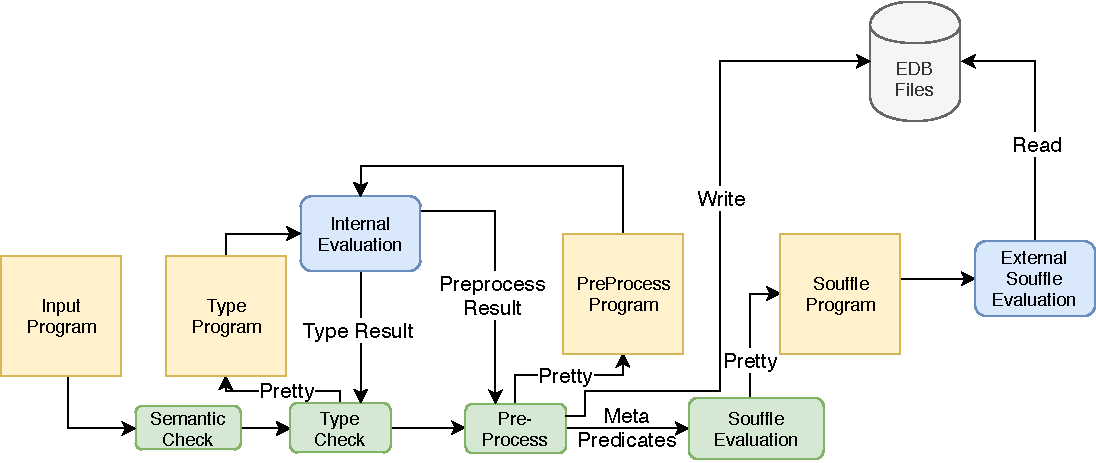
\includegraphics[scale=0.65]{./souffleEval.pdf}
\end{figure}
\end{frame}

\begin{frame}[fragile]{}

\begin{overprint}
\onslide<1>
\centering\fbox{Actual Code for Person Program}
\begin{minted}[
frame=lines,
framesep=2mm,
bgcolor=bg,
]{haskell}
EDB('Parent, "Parent.csv").
TYPEOF('Parent, [String String]).
OUTPUT('Ancestor).
Ancestor(p, c) :- Parent(p, c).
Ancestor(a, c) :- Parent(p, c), Ancestor(a, p).
\end{minted}
\onslide<2>
\centering\fbox{Souffle Code for Person Program}
\begin{minted}[
frame=lines,
framesep=2mm,
bgcolor=bg,
]{haskell}
.decl Ancestor(x_0:symbol, x_1:symbol)
.decl Parent(x_0:symbol, x_1:symbol)
.decl EDB(x_0:symbol, x_1:symbol)
.decl OUTPUT(x_0:symbol)
.decl TYPEOF(x_0:symbol, x_1:symbol)
.input Parent(filename="Parent.csv", delimiter=",")
.input EDB(filename="EDB.csv", delimiter=",")
.input TYPEOF(filename="TYPEOF.csv", delimiter=",")
.input OUTPUT(filename="OUTPUT.csv", delimiter=",")
.output Ancestor(delimiter=",")
Ancestor(p, c) :- Parent(p, c).
Ancestor(a, c) :- Parent(p, c), Ancestor(a, p).
\end{minted}
\end{overprint}
\end{frame}
\def\checkmark{\tikz\fill[scale=0.4, color=green](0,.35) -- (.25,0) -- (1,.7) -- (.25,.15) -- cycle;} 

\begin{frame}
\frametitle{Comparison Against Souffle 
\includegraphics[width=20pt]{souffle.png}}
\begin{itemize}
	\item<1-> Souffle has no type inference
	\item<2-> Souffle has no meta-predicates
	\item<3-> ... But it does have aggregates (COUNT, MIN, MAX, ...)
	\item<4-> ... More advanced type system that permits definition of new types.
	\item<5-> ... Lots of built-in functions (e.g. strlen, substr, ...)
	\item<6-> The naive internal evaluation strategy shows $\mathcal{O}(N^4)$ behavior for $N$ linear descendants in the ancestor example (matches theoretical result for naive algorithm)
	\item<7-> ... Souffle shows $\mathcal{O}(N^{2 + \epsilon})$, $\epsilon \approx 0.3$. 
	\item<8-> Optimal is $\binom{N}{2} = \mathcal{O}(N^2)$ (total size of Ancestor Relation)
\end{itemize}
\end{frame}

\begin{frame}

\centering \Huge Questions?

\end{frame}
% etc
\end{document}
